\documentclass[modern, trackchanges, dvipsnames]{aastex631}
  \urlstyle{sf}


\usepackage{CJK}
\usepackage{microtype}
\usepackage{savesym}
  \savesymbol{lambdabar}
\usepackage{newpxtext, eulerpx}
  \restoresymbol{newpx}{lambdabar}
\usepackage[T1]{fontenc}
\usepackage{fontawesome}
\usepackage{amsmath}
\usepackage{bm}
\usepackage{nicefrac}
\usepackage[caption=false]{subfig}
\usepackage[figure,figure*]{hypcap}
%\usepackage{tikz}
%  \usetikzlibrary{positioning, fit, calc, arrows.meta}
\usepackage{booktabs}


\newcommand{\pmwd}{{\usefont{T1}{nova}{m}{sl}pmwd}}
\newcommand{\GADGET}{{{\fontsize{10pt}{12pt}\selectfont GADGET}-4}}
\newcommand{\GSDATA}{{GS512}}

%\renewcommand{\sectionautorefname}{Sec.}
%\renewcommand{\subsectionautorefname}{Sec.}
%\renewcommand{\appendixautorefname}{App.}
%\renewcommand{\figureautorefname}{Fig.}
%\newcommand{\subfigureautorefname}{\figureautorefname}

%FIXME copied from ../adjoint/adjoint.tex
\newcommand{\deltaD}{\delta^\textsc{d}}
\newcommand{\deltaK}{\delta^\textsc{k}}
\renewcommand{\d}{d}
\newcommand{\p}{\partial}
\newcommand{\cJ}{\mathcal{J}}
\newcommand{\cR}{\mathcal{R}}
\newcommand{\cL}{\mathcal{L}}
\newcommand{\cH}{\mathcal{H}}
\bmdefine{\vzero}{0}
\bmdefine{\vI}{I}
\bmdefine{\vnabla}{\nabla}
\bmdefine{\vtheta}{\theta}  % parameters
\bmdefine{\vvartheta}{\vartheta}  % relevant scales and factors to form
                                  % dimensionless features as NN inputs
\bmdefine{\vomega}{\omega}  % white noise modes
\bmdefine{\vk}{k}  % wavevectors
\bmdefine{\vx}{x}  % comoving and canonical coordinates
\bmdefine{\vq}{q}  % Lagrangian coordinates
\bmdefine{\vs}{s}  % displacements
\bmdefine{\vp}{p}  % canonical momenta
\bmdefine{\vv}{v}  % FIXME some velocities
\bmdefine{\va}{a}  % accelerations
\bmdefine{\vz}{z}  % states
\bmdefine{\vo}{o}  % observable
\bmdefine{\vf}{f}
\bmdefine{\vF}{F}
\bmdefine{\vDelta}{\Delta}
\bmdefine{\vLambda}{\Lambda}
\bmdefine{\vlambda}{\lambda}
\bmdefine{\vvarphi}{\varphi}
\bmdefine{\vxi}{\xi}  % x adjoint
\bmdefine{\vpi}{\pi}  % p adjoint
\bmdefine{\valpha}{\alpha}  % force vjp x gradient
\bmdefine{\vzeta}{\zeta}  % force vjp theta gradient
\newcommand{\lna}{\ln\!a}
\newcommand{\lnk}{\ln\!k}
\newcommand{\half}{\nicefrac12}
\newcommand{\As}{A_\mathrm{s}}
\newcommand{\ns}{n_\mathrm{s}}
\newcommand{\Omegam}{\Omega_\mathrm{m}}
\newcommand{\Omegab}{\Omega_\mathrm{b}}
\newcommand{\Mpc}{\mathrm{Mpc}}
\newcommand{\ic}{\mathrm{i}}
\newcommand{\linear}{\mathrm{lin}}
\newcommand{\tophat}{\mathrm{TH}}
\newcommand{\gauss}{\mathrm{G}}

\newcommand{\GPU}{NVIDIA H100 PCIe}  % 80GB memory

\newcommand{\YL}[1]{\textcolor{Bittersweet}{#1}}
\newcommand{\YZ}[1]{\textcolor{MidnightBlue}{#1}}



\begin{document}



\title{\large Neural and Symbolic Optimization of Cosmological
Particle-Mesh Simulation
\vspace{0.3em}}


\author[0000-0002-9300-2632]{\normalsize Yucheng Zhang}
\affiliation{Department of Mathematics and Theory, Peng Cheng
Laboratory, Shenzhen, Guangdong 518066, China}
\affiliation{Center for Cosmology and Particle Physics, New York
University, New York, New York 10003, USA}

\author[0000-0002-0701-1410]{\normalsize Yin Li}
\affiliation{Center for Computational Mathematics, Flatiron Institute,
New York, New York 10010, USA}
\affiliation{Department of Mathematics and Theory, Peng Cheng
Laboratory, Shenzhen, Guangdong 518066, China}
\affiliation{Center for Computational Astrophysics, Flatiron Institute,
New York, New York 10010, USA}

\author[0000-0001-5044-7204]{\normalsize Drew Jamieson}
\affiliation{Max Planck Institute for Astrophysics, 85748 Garching bei
M\"unchen, Germany}

\author[0000-0003-0745-9431]{\normalsize Libin Lu}
\affiliation{Center for Computational Mathematics, Flatiron Institute,
New York, New York 10010, USA}


\shorttitle{Optimized Cosmological Simulation}
\shortauthors{Zhang \& Li et al.}


\correspondingauthor{Yucheng Zhang \& Yin Li}
\email{yucheng.zhang@nyu.edu \& eelregit@gmail.com}



\begin{abstract}
% up to 150 words

We optimize the spatial resolution of cosmological particle-mesh (PM)
simulations by sharpening the PM force with first neural networks and then
symbolic regression, taking symmetry and dimensional analysis in consideration.

We combine differentiable simulation, deep learning, [decision tree
(feature selection)], and symbolic regression to extract the final kernel
applicable to all other cosmological simulation code.

\end{abstract}



\section*{TODO}
\begin{itemize}
\item (paper) Moving some of the following ongoing and completed tasks
  to the main text and add preliminary figures.
\item (data; YL) Incorporate 3lpt branch; testing; find a\_start for
  different mass resolutions; probably replace linear snapshot spacing
  according to the nonlinearity (estimate (with PM till convergence) the
  std acc over the std vel) of each realization.
\item (model; YL) Change nbody for loop by lax scan and/or while loops.
  while\_loop can help to save compilation when trained on different
  snapshots. Performance difference between scan and while?\newline
  \YZ{It seems that lax.while\_loop only supports fwd grad}
  \href{https://jax.readthedocs.io/en/latest/notebooks/Common_Gotchas_in_JAX.html#summary}{link}
\item (model; YL) Compare one pair of \GADGET\ and \pmwd\ (with say 100 to 1000 time
    steps) results and make sure that they agree perfectly on the large
    scales. For this purpose the box size should be large enough (in
    linear regime), say 1 Gpc/$h$.\newline
    \YZ{\textbf{Update}: for Sobol=6, boxsize=983Mpc, \GADGET\ and \pmwd\ are
    visually consistent at the field level. For power spectrum: For
    odd mesh shapes (e.g. 1, 3, 5), pmwd and \GADGET\ are perfectly consistent
    on large scales. \textbf{While for even mesh shapes (e.g. 2, 4), the powers
    look slightly different. To figure out this weird issue.}}
\item (model; YL) Probably necessary to first incorporate List \& Hahn's
  recent improvement on FastPM integrator arXiv:2301:09655.
\item (train, test) For $\vs(\vq)$, $\vv(\vq)$, $\delta(\vx)$,
  $(1+\delta)\vv(\vx)$, $(1+\delta)\vv\vv(\vx)$, show $T - 1$ in symlog
  with 0.01 linthresh, and $1-r^2$ in log at 3 different $a$'s; Show $f$
  and $g$ (along axis and face diagonal) at 3 different $a$'s
\item (train, test) 3 sets of grid for ptcl, force mesh, and loss. Add
  random offset in loss grid (see \autoref{tab:param}) to remove the
  position dependence in loss; likewise for force mesh? how about only
  training (for lower loss), only ``inference'' (for higher accuracy),
  or both? the random force mesh offset can also be replaced by a
  structured scheme, e.g., alternating between 2 interlocking grids
\item (train) Explore if we can use a finer loss grid, from 1x to say
  1.5x and even 2x.
\item (train, test) Non-integer multiple mesh shapes: for uniform
  particle grid, test (with double precision on CPUs) whether they start
  moving by artifact forces on cell scales, in 3 cases: no
  deconvolution, with CIC deconvolution, with SO.
\item (train) find the best loss function for production training
\item (train) For generalizability and robustness, consider testing
  weight decay and dropout. Also they're worth adding if they give lower
  losses at convergence. Note that 512 realization are not too many, and
  we have features that can be very correlated.\newline
  \YZ{Dropout with Flax has been coded. We can use Optax AdamW for weight decay.}
\item (train) optuna hyperparam search on a subset of training data
  before production training
  (\href{https://github.com/optuna/optuna-examples/blob/main/haiku/haiku_simple.py}{optuna
  example}).\newline
  \YZ{Do we also use another subset of the training data as validation data?}
\item (train) Reduce learning rate on (mean epoch) loss plateau in
  production\newline
  \YZ{A simple scheduler has been coded, to be fine-tuned for production training.}
\item (test) Interpolation test: compare SO DM and halo fields and
  summary stats with those of raw pmwd, deconvolved pmwd, and \GADGET,
  on the last 9 test cases and noncubic box.
\item (test) Extrapolation test: demonstrate generalization capability,
  compare extrap PySR, extrap SO, raw pmwd, deconv pmwd, and \GADGET.
\item (test) Generate a sample of $(X, y)$ data with the trained neural network
  for feature selection and symbolic regression.
\item \YZ{Do we also consider pruning and distilling of the trained networks?}
\item (paper) Think about what figures and tables to show in the paper. Up
to 6 items could be included. Some tables could be included in the context as
list if we have too many figures to show?\newline
  \YZ{figures:
  1. $f$ and $g$ functions, both NN and Symbolic.
  2. Density field (and halo?) with zoom in for small scale sharpening.
  3. Transfer function and correlation coefficient.
  4. Halo related stats.}
\item Fix cross references and other journal quirks as a patch
\end{itemize}


% Main text: up to 3500 words: introduction + results + discussion
% so we should keep introduction and discussion brief
\vspace{1em}
\section{Introduction}
% without heading

Abbrs: vector-Jacobian product (VJP), automatic differentiation (AD), neural
network (NN), particle-mesh (PM), fast-Fourier transform (FFT)

% AI for science and cosmology

% a brief review of (differentiable) cosmological simulations
BORG, ELUCID, and BORG-PM \citep{BORG, ELUCID, BORG-PM}
\texttt{FastPM} and \texttt{FlowPM} \citep{FastPM, vmad, SeljakEtAl2017, FlowPM}


% introduce PM and its limitation on small scales
The PM method solves the Poisson equation by scattering the particles onto a
mesh, on which FFT is performed and the Laplacian operator reduces to simple
multiplication of wavenumbers in Fourier space.
Although being computationally efficient, the PM method is mainly limited by its
resolution on small scales, i.e. scales around the mesh cell size.
This is due to the loss of information during the scattering process of
continuously distributed particles onto the discrete mesh.
We use the cloud-in-cell (CIC) scheme \citep{HockneyEastwood1988} to compute the
mass fractions of a particle scattered to nearby grid points.
Other schemes include the nearest grid point (NGP) and triangle shaped cloud
(TSC) etc.

Using a hybrid embedding of NNs in differentiable physical simulations, we
optimize the performance of PM method on small scales in cosmological $N$-body
simulations by sharpening the gravitational force.


\vspace{1em}
\section{Results}
% Results should be divided by topical subheadings
% Put main ideas in Results first, then more technical details in Methods.

\subsection{Optimization of Dynamics}

\begin{table}
  \centering
  \caption{Possible features that can affect force sharpening.
  All scales are then multiplied by the wavenumber $k$ to form dimensionless
  factors.}
  \label{tab:feat}
  \begin{tabular}{rl}
  \toprule
  type & feature \\
  \midrule
  & $R_\mathrm{d}$: RMS linear displacement \\
  \cmidrule(lr){2-2}
  & $R_P$: $\Delta_\linear^2(R_P^{-1}) \triangleq 1$ \\
  \cmidrule(lr){2-2}
  nonlinear scales & $R_\tophat$: $\sigma_\tophat^2(R_\tophat) \triangleq 1$ \\
  \cmidrule(lr){2-2}
  & $R_\gauss$: $\sigma_\gauss^2(R_\gauss) \triangleq 1$ \\
  \cmidrule(lr){2-2}
  & $\d R / \d\lna$: time derivatives of the above \\
  \midrule
  & particle spacing \\
  \cmidrule(lr){2-2}
  other scales & $l$: PM force mesh cell size \\
  \cmidrule(lr){2-2}
  & softening length \\
  \midrule
  & $G_m(a) \triangleq D_m(a) / a^m, m \in \{1, 2, \YL{3's?}\}$ \\
  \cmidrule(lr){2-2}
  & $\d\ln G_m / \d\lna$ \\
  \cmidrule(lr){2-2}
  dimensionless factors & $\Omegam(a)$ \\
  \cmidrule(lr){2-2}
  & $\d\ln\!H / \d\lna$ \\
  \cmidrule(lr){2-2}
  & $\Delta\lna$: time step size in $\lna$ \\
  \bottomrule
  \end{tabular}
  \end{table}

In cosmological $N$-body simulations, the dynamics of the particles is governed
by the Poisson equation
%
\begin{equation}
  \nabla^2 \varphi(\vx) = \frac32 \Omegam H_0^2 \delta(\vx),
\end{equation}
%
In Fourier space, the gravitational force field $- \vnabla \varphi$ reads
%
\begin{equation}
- i \vk \varphi(\vk) = i \frac32 \Omegam H_0^2 \,\frac{\vk}{k^2} \delta(\vk),
\end{equation}
%
where we introduce force sharpening for spatial optimization through
%
\begin{equation}
\frac{i k_i}{k^2} \to \frac{i k_i}{k^2}
  f(k_i; \vvartheta) g(k_1, k_2, k_3; \vvartheta),
\end{equation}
%
where $f$ and $g$ are NNs, each approximating a nonlinear function of the
wavevector components and all possible relevant features $\vvartheta$ summarized
in \autoref{tab:feat} with more details discussed in \autoref{sec:features}.
Gravity obeys the $\mathrm{O}(3)$ rotational symmetry, which is however
broken by the PM solver to the O\textsubscript{h} discrete symmetry with
48 elements involving permutations and reversals of the 3 principal axes
of the simulation box.
The PM evaluation of each force component can further break the symmetry
along that axis, leaving the remaining 2 permutationally symmetric.
Therefore, we implement $f$ and $g$ to be even functions of the
wavevector components, and $g$ to be permutation equivariant in all 3
components, so that $f g$ is the most general modification to the force
kernel.
An even and real kernel in configuration space is also even in Fourier
space.
We take the absolute value for the evenness, and sort the 3 wavevector
compontents to achieve the permutation equivariance.
Being embedded in the differentiable simulation, the NNs can be trained using
gradient-based optimization methods as in usual deep learning tasks.
The parameters of the neural networks, which enter the force evaluation in
every time integration step, can be treated just the same as other cosmological
parameters.
The objective gradients are accumulated, based on which the parameters are then
optimized.
For both $f$ and $g$ neural networks, we adopt multilayer perceptron (MLP, i.e.
fully connected) structures.


\begin{table*}
  \centering
  \caption{Ranges of \GADGET\ and \pmwd\ configuration and cosmological
  parameters.
  Note that the grid ratio need next fast len to determine the mesh shape
  for fast FFT.
  Given the box size, the mesh shape determines the cell size.
  The softening parameter gives the ratio of the comoving softening length
  to the mean particle spacing.
  The curvature $\Omega_k$ is related to the separate universe simulation.
  We sample parameters applicable to \GADGET\ during data generation, and
  those applicable to \pmwd\ during training.
  \textsuperscript\dag{}The box size is determined jointly by the \pmwd\
  mesh shape and mesh cell size below, which are assumed to be sampled
  independently.
  \YL{I forgot why I wrote ``Mpc'' without the $h$ here.}
  \YZ{We are using ``Mpc/h'' in the code.}
  In practice, we sample one conditioned on the other and the box size.
  *Number of time steps from $a=1/16$ to $a=1+1/128$ (in order to cover the
  snapshot offset).
  }
  \label{tab:param}
  \begin{tabular}{lcccr}
  \toprule
  applicability & parameter & distribution & range & sampling \\
  \midrule
  & $128^3$ white noise & $\mathcal{N}(\vzero, \vI)$ & 512 realizations & MC \\
  \cmidrule(lr){2-5}
  & 121 snapshots, $a$ & uniform & [1/16, 1] & deterministic \\
  \cmidrule(lr){2-5}
  & box size in Mpc\YZ{/h}\textsuperscript\dag & log-trapezoidal & [25.6, 2560) \\
  \cmidrule(lr){2-4}
  & snapshot offset, $\Delta\!a$ & uniform & [0, 1/128) \\
  \cmidrule(lr){2-4}
  \GADGET\ & $\As \times 10^9$ & log-uniform & [1, 4) \\
  \cmidrule(lr){2-4}
  \& \pmwd\ & $\ns$ & log-uniform & [0.75, 1.25) & RQMC \\
  \cmidrule(lr){2-4}
  & $\Omegam$ & log-uniform & [1/5, 1/2) & see \autoref{fig:sobol} \\
  \cmidrule(lr){2-4}
  & $\Omegab / \Omegam$ & log-uniform & [1/8, 1/4) \\
  \cmidrule(lr){2-4}
  & $\Omega_k / (1 - \Omega_k)$ & uniform & [-1/3, 1/3) \\
  \cmidrule(lr){2-4}
  & $h$ & log-uniform & [0.5, 1) \\
  \cmidrule(lr){1-4}
  \GADGET\ & softening ratio & log-uniform & [1/50, 1/20) \\
  \cmidrule(lr){1-5}
  & mesh shape & log-uniform & [128, 512] \\
  \cmidrule(lr){2-4}
  \pmwd\ & mesh cell size in Mpc\YZ{/h} & log-uniform & [0.2, 5] & MC \\
  \cmidrule(lr){2-4}
  & number of time steps* & log-uniform & [10, 1000] \\
  \cmidrule(lr){1-4}
  training & loss grid offset in its own spacing & uniform & $[0, 1)^3$ \\
  \bottomrule
  \end{tabular}
  \end{table*}

We generate our target data for training and testing with the \GADGET\
simulation code \citep{GADGET-4}.
We run 512 \GADGET\ simulations that cover a wide range of
configurations and cosmological parameters, as listed in
\autoref{tab:param}.
Each simulation has $128^3$ particles and writes 121 snapshots linearly
spaced in scale factor from $1/16 + \Delta a$ to $1 + \Delta a$, with
spacing $1/128$.
$\Delta a$ is an offset, common for all snapshots in each simulation,
that varies as in \autoref{tab:param} and helps to sample different
alignment between snapshot and start/stop times.
In our \pmwd\ model, we generate the snapshot at an arbitrary given time using
the cubic Hermite interpolation, with more details in \autoref{sec:snapobs}.
The curvature $\Omega_k$ is related to the separate universe simulation
\citep{LiEtAl2014, WagnerEtAl2015}.
\YZ{We refer to this training dataset of 512 \GADGET\ simulations sampled with
Sobol sequence as \GSDATA.}
On average each \GADGET\ simulation takes roughly 2K CPU hours to run, and the
generation of the whole \GSDATA\ dataset consumes 1M CPU hours.
% to be compare with the speed of pmwd with SO


\subsection{Trained Neural Networks}

% visualization & comparison of neural nets & symbolic functions
For the $f(k_i; \vvartheta)$ NN, we show it as a function of $k_i$ at multiple
different $\vvartheta$ values.

For the $g(k_1,k_2,k_3;\vvartheta)$ NN, which is permutationally symmetric about
$(k_1, k_2, k_3)$, we show it as a function of $k_i$ along axis and face
diagonal directions.


\subsection{Feature Importance}

We generate a sample of (input, output) data of the trained neural network to
perform feature importance analysis.
We use Sobol sequence to generate the sample of (parameters in
\autoref{tab:param}, $k$, $a$).

We use the random forest regressor for feature selection using impurity-based
importance.
We use the \texttt{scikit-learn} \citep{scikit-learn} code for this.
% more details on the hyperparams in random forest
\YZ{Maybe we can add another column in \autoref{tab:feat} for feature
importance?}


\subsection{Symbolic Expressions}

The selected important features are then used for SR.
We use the \texttt{PySR} \citep{PySR} SR code to fit for analytic
function expressions of the trained SO neural networks.


\subsection{Dark Matter Density Fields}

\begin{figure*}
  \centering
  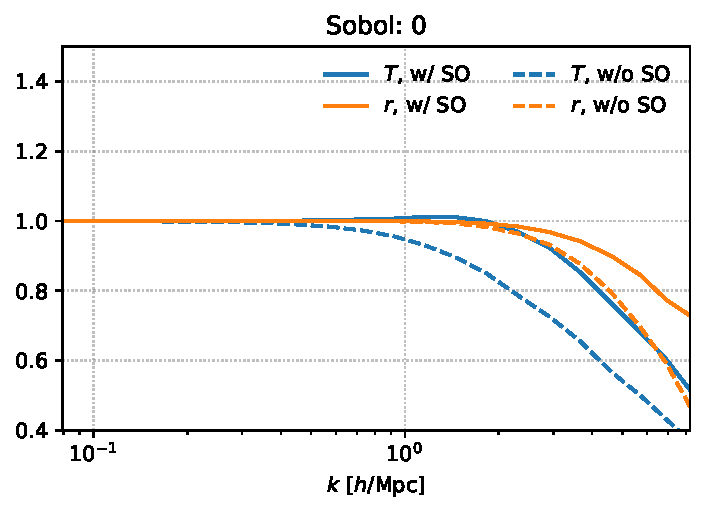
\includegraphics[width=.8\columnwidth]{sobol0snap120epoch300.pdf}
  \caption{The transfer function $T$ and correlation coefficient $r$ of the
  \GADGET\ and \pmwd\ simulated density fields, with and without force
  sharpening.
  Sobol 0 snap 120}
  \label{fig:tfcc}
\end{figure*}

% transfer function & correlation coefficient
To compare two fields $\hat f$ and $f$, we introduce for each mode the square
root ratio of power
%
\begin{equation}
T(\vk) \triangleq
\sqrt{\frac{|\hat f(\vk)|^2}{|f(\vk)|^2}},
\label{T}
\end{equation}
%
which is also referred to as the transfer function, and the cross correlation
coefficient
%
\begin{equation}
r(\vk) \triangleq
\frac{\Re \bigl[ \hat f(\vk) f^*(\vk) \bigr]}
     {\sqrt{|\hat f(\vk)|^2 |f(\vk)|^2}}.
\label{r}
\end{equation}
%
The two fields are identical when both $T$ and $r$ are unity.
The PM method is accurate on scales much larger than the cell size, therefore we
expect $T$ and $r$ to be very close to being unity both before and after force
sharpening optimization.



\begin{figure*}
  \centering
  \includegraphics[width=.8\columnwidth]{denslab_0_120_e300.pdf}
  \caption{Projected dark matter density fields of \GADGET, \pmwd\ without and
  with force sharpening.
  Sobol 0 snap 120}
  \label{fig:denslab}
\end{figure*}

% density field with zoom in (with halos painted as circles?)
The effect of force sharpening can also be visually shown by looking directly at
the density field.


\subsection{Dark Matter Halo Catalogs}


\vspace{1em}
\section{Discussion}
% Discussion does not contain subheadings


\vspace{1em}
\section{Methods}


\vspace{1em}
\subsection{Differentiable Simulation}
\label{sec:pmwd}

The differentiable cosmological simulation with adjoint method \citep{Li2022a}
and the corresponding PM $N$-body library \pmwd\ \citep{Li2022b} are the
foundation of the gradient-based optimization discussed in this work.
Within this fully differentiable framework, we are able to embed neural networks
in physical processes and train them for many purposes, including the
optimization of spatial resolution by sharpening the gravitational force in this
work.

Here we briefly recap the equations that are closely related to our
extensions to the original framework, and setup the notations of the variables.
Following \cite{Li2022a}, we denote the particles' state with $\vz = (\vx,
\vp)^\intercal$ and their adjoint variables with $\vlambda = (\vxi, \vpi)$.
We refer to the quantities that are directly related to the final objective
function $\cJ$ as the observable $\vo$.
In this work, our observable includes multiple snapshots at given times.
For the observation operator $O_{i}^{i-1}$ in the adjoint equations (check
Eq.(18) in \cite{Li2022a}) from time step $a_i$ back to $a_{i-1}$, the adjoint
variables are updated through
\begin{align}
  \vxi_{i-1} &:= \vxi_{i-1} + \frac{\p\cJ}{\p\vo}\frac{\p\vo}{\p \vx_{i-1}}, \nonumber\\
  \vpi_{i-1} &:= \vpi_{i-1} + \frac{\p\cJ}{\p\vo}\frac{\p\vo}{\p \vp_{i-1}},
\end{align}
where the derivatives of $\vo$ with respect to $\vx_{i-1}$ and $\vp_{i-1}$ would
be non-zero only if they were used in the generation of any snapshots in $\vo$.
The initial conditions of these adjoint variables are given by
\begin{align}
  \vxi_n &= \frac{\p\cJ}{\p\vo}\frac{\p\vo}{\p\vx_n}, \nonumber\\
  \vpi_n &= \frac{\p\cJ}{\p\vo}\frac{\p\vo}{\p\vp_n},
\end{align}
which are zero if no snapshot in $\vo$ depends on $(\vx_n, \vp_n)$.
The derivative of the objective function with respect to the observable
($\p\cJ/\p\vo$) and the VJPs of the observation operation ($\p\vo/\p\vx_n$ and
$\p\vo/\p\vp_n$, mainly the interpolation function discussed in
\autoref{sec:snapobs} below) can be conveniently computed by AD.


\vspace{1em}
\subsection{Snapshot Observable}
\label{sec:snapobs}

The N-body time integration is carried out following discrete time steps. Given
the particle displacements $\vx$ and velocities $\vv = \vp/(a^3H)$ at two
consecutive time steps $a_i$ and $a_{i+1}$, we get the snapshot of particles in
between at $a$ using
the cubic Hermite interpolation.
The interpolated particle displacements are given by
\begin{align}
  \vx(a) =\ &h_{00}(\alpha)\vx_i + h_{10}(\alpha)(a_{i+1} - a_i)\vv_i + \nonumber\\
           &h_{01}(\alpha)\vx_{i+1} + h_{11}(\alpha)(a_{i+1} - a_i)\vv_{i+1},
\end{align}
where $\alpha := (a - a_i)/(a_{i+1} - a_i)$ and the Hermite basis functions read
\begin{align}
  h_{00}(\alpha) &= 2\alpha^3 - 3\alpha^2 + 1, \nonumber\\
  h_{10}(\alpha) &= \alpha^3 - 2\alpha^2 + \alpha, \nonumber\\
  h_{01}(\alpha) &= -2\alpha^3 + 3\alpha^2, \nonumber\\
  h_{11}(\alpha) &= \alpha^3 - \alpha^2.
\end{align}
The particle velocities are then given by the derivative $\d\vx / \d a$.
Note that the interpolation is a linear combination of the particle snapshots at
two consecutive time steps, which therefore can be done in either two steps or
just one step by carrying the particles from the previous time step.
We find the two-steps scheme more convenient for the backward evolution of the
adjoint variables.
The interpolated snapshots at different times make the observable in this work,
and the VJPs of the interpolation operation are computed by AD and put into the
adjoint equations as mentioned in \autoref{sec:pmwd}.


\vspace{1em}
\subsection{Input Features}
\label{sec:features}

Multiple scales and dimensionless factors could possibly affect force
sharpening, which are denoted as $\vvartheta$ and enter the NNs of $f(k_i;
\vvartheta)$ and $g(k_1, k_2, k_3; \vvartheta)$ as input features.
A list of these features is summarized in \autoref{tab:feat}, and here we
present relevant definations and more details.

Below are some definations related to the typical scales.
\begin{itemize}
\item The root-mean-square (RMS) linear displacement is given by
%
\begin{equation}
R_\mathrm{d} = \int \frac{k P_\linear(k)}{6\pi^2} \d\lnk,
\end{equation}
%
where $P_\linear(k)$ is the linear power spectrum.
\item The dimensionless linear power spectrum is defined as
%
\begin{equation}
\Delta^2_\linear(k) \triangleq \frac{k^3 P_\linear(k)}{2 \pi^2},
\end{equation}
%
based on which we define a nonlinear scale $R_P$ through
$\Delta_\linear^2(R_P^{-1}) \triangleq 1$.
\item The variance of linear matter overdensity in a top-hat window is given by
%
\begin{equation}
\sigma_\tophat^2(R) = \int_0^\infty \frac{\d k}k
  \Delta_\linear^2(k) W_\tophat^2(kR),
\end{equation}
%
where $W_\tophat(kR) = 3[\sin(kR) - kR\cos(kR)] / (kR)^3$ is the
Fourier transform of the top-hat window.
Then we have $R_\tophat$: $\sigma_\tophat^2(R_\tophat) \triangleq 1$.
\item Likewise $\sigma_\gauss^2(R)$ is defined with a Gaussian window
$W_\gauss(kR) = e^{-(kR)^2/2}$, and $R_\gauss$: $\sigma_\gauss^2(R_\gauss)
\triangleq 1$.
\end{itemize}
These nonlinear scales are functions of time since the linear power spectrum
evolves with time through the growth factor $D(a)$, we also take the time
derivatives of these scales as input features.
Other relevant scales include the particle spacing in Lagrangian space, the cell
size of the chosen mesh grid for force evaluation, and the softening length in
the target \GADGET\ simulations.

Relevant scale-independent dimensionless factors are
\begin{itemize}
\item $G_m(a) \triangleq D_m(a) / a^m$: linear growth given in
  suppression factors for $m \in \{1, 2\}$;
\item $\d\ln G_m / \d\lna$: with $m=1$ case related to the growth rate
  $f \triangleq \d\ln D_1 / \d\lna$;
\item $\Omegam(a)$: matter density parameter at $a$;
\item $\d\ln\!H / \d\lna$: time derivative of Hubble expansion;
\item $\Delta\lna$: time step size in $\lna$.
\end{itemize}

Dimensionless combinations are formed by multiplying the wavevector components
with the scales, i.e.,
%
\begin{equation}
f(k_i; \vvartheta) = f(k_iR_d, k_iR_P, \cdots; G_m, \Omegam, \cdots),
\end{equation}
%
\begin{equation}
g(k_1, k_2, k_3; \vvartheta) = g(\{k_jR_d, k_jR_P, \cdots\}_{j=1,2,3}; G_m, \Omegam, \cdots).
\end{equation}
%


\vspace{1em}
\subsection{Loss Function}
\label{sec:loss}

The loss function is constructed by comparing the simulated field $\hat f$ with
the target field $f$.
\YL{
For a field $f$ in either Lagrangian or Eulerian space, we have thought
of 3 forms of MSE-inspired loss:
%
\begin{equation}
\cL_f = \frac1{N_a} \ln
  \frac{\sum_\vq \bigl[ \hat f(\vq) - f(\vq) \bigr]^2}
       {\sum_{\vq'} f(\vq')^2},
\end{equation}
%
where $N_a$ is the number of time steps it takes to generate the snapshot for
each iteration
(or with $\vq$ replaced by $\vx$ for Eulerian fields, or equivalently by
their Fourier wavevector $\vk$ in both cases).
%
\begin{equation}
\cL_f = \frac1{N_K N_a} \sum_{ij} \ln \biggl[
\frac{\sum_{\vk \in K_i} \bigl| \hat f(\vk, a_j) - f(\vk, a_j) \bigr|^2}
     {\sum_{\vk' \in K_i} | f(\vk', a_j)|^2} + \epsilon \biggr],
\end{equation}
%
where $\epsilon$ sets the relative threshold tolerance below which we
consider $\hat f$ in each $K$ accurate enough, and the gradients from
that bin unimportant.
%and
%%
%\begin{equation}
%\cL_f = \frac1{N_a} \ln \biggl[ \frac1{N_K} \sum_i
%\frac{\sum_{k \in K_i} w(\vk)
%      \bigl| \hat f(\vk) - f(\vk) \bigr|^2}
%     {\sum_{k' \in K_i} |f(\vk')|^2} \biggl].
%\end{equation}
%%
Then the question is which loss we should use for which $f$, to get
stable and robust results, e.g., no bump for large or small boxes.
To further limit our scope in this paper, we should probably only
consider $f \in \{\vs, \delta\}$, and optionally the Lagrangian particle
velocity $\vv(\vq)$.
}

For the displacement field, we adopt the mean squared error (MSE) loss
that proved effective in many previous works
\citep[e.g.,][]{HeEtAl2019, LiEtAl2021}:
%
\begin{equation}
\cL_\vs = \ln \frac{\sum_\vq \bigl[ \hat\vs(\vq) - \vs(\vq) \bigr]^2}
                   {\sum_{\vq'} s(\vq')^2},
\end{equation}
%
in which a particle originating from its Lagrangian position $\vq$ is
displaced by $\vs$ in the \GADGET\ snapshot and by $\hat\vs$ in the
prediction of \pmwd\ model in training.
Note that we have further taken the logarithm to combine it with the
other loss(es) below.
% Say that only s loss is not enough even though in principle it is, and cite DrewEtAl x2 too

\YL{Even though the log should be enough for adaptive optimizer and
fixed sim config, this may create problem when training on all config at
the same time. So normalizations inside the log is added above and
below.}

However, in the Eulerian space, an MSE loss is dominated by the small
scale modes.
In this work we choose uniform weights in the scale space on the
relative MSE.
We bin the modes logarithmically by \nicefrac13 octave in scale, with
the $i$-th $k$-bin $K_i \triangleq [k_i, k_{i+1})$, where $k_i =
2^{1+i/3} \pi / L$.
Our loss on the overdensity field $\delta$ sums up its MSE relative to
the target field power in logarithmic bins:
%
\begin{equation}
\cL_\delta = \frac1{N_K} \sum_i \ln
\frac{\sum_{k \in K_i} \bigl| \hat\delta(\vk) - \delta(\vk) \bigr|^2}
     {\sum_{k' \in K_i} |\delta(\vk')|^2},
\end{equation}
%
\begin{equation}
\cL_\delta = \frac1{N_K} \sum_i
\frac{\sum_{k \in K_i} w(\vk)
      \bigl| \hat\delta(\vk) - \delta(\vk) \bigr|^2}
     {\sum_{k' \in K_i} |\delta(\vk')|^2},
\end{equation}
%
where $N_K$ is the number of $k$-bins and $w(\vk)$ is a nonnegative
factor that suppresses the high $k$ contribution in Eulerian fields such
as the density field (with $w=1$ for the Lagrangian displacement field).
This is because a PM solver gradually loses small scale information step
by step, and without $w$ setting the priority, the loss function could
encourage the network to fit the small scales at the cost of the
intermediate scales.
Note that $\cL_\vs$ is on the displacement field $\vs(\vq)$ in the
Lagrangian space, while the density field is in the Eulerian space:
%
\begin{equation}
1 + \delta(\vx) = \int\!\d^3\vq\, \deltaD[ \vx - \vq - \vs(\vq)],
\end{equation}
%
which we compute by scattering particles to the choice of grid for loss.

Under the mild assumptions that $T$ \eqref{T} and $r$ \eqref{r} are smooth
and isotropic, we can show
%
\begin{equation}
\cL_\delta \propto \int \!\d\ln\!k\, \ln
\Bigl\{ \bigl[ 1 - T(\vk) \bigr]^2
  + 2 T(\vk) \bigl[ 1 - r(\vk) \bigr] \Bigr\} \geq -\infty,
\end{equation}
%
replacing
%
\begin{equation}
\cL_\delta \propto \int \!\d\ln\!k\, w(\vk)
\Bigl\{ \bigl[ 1 - T(\vk) \bigr]^2
  + 2 T(\vk) \bigl[ 1 - r(\vk) \bigr] \Bigr\} \geq 0,
\end{equation}
%
that only vanishes when both $T$ and $r$ are unity for all modes, i.e.,
when $\hat\delta$ is identical to $\delta$.
Above we choose the binned version instead for the robustness against
the noisy modewise $|\delta(\vk)|^2$ in the denominator.
The derivation here is similar to that in \citet{HeEtAl2019} on the MSE
loss, while our modification is important to balance among all scales so
that the neural network does not focus too much on either high or low
$k$'s.

We combine Lagrangian and Eulerian fields to form the total loss for a single
snapshot:
%
\begin{equation}
\cJ = \cL_\vs + \cL_\delta.
\end{equation}
%

\YZ{We further sum the loss of all snapshots across a single forward simulation
at different times, i.e.
\begin{equation}
\cJ = \sum_{a_i} \cJ |_{a_i}
\end{equation}
}


\vspace{1em}
\subsection{Configurations and Training Data}

\begin{figure*}
  \centering
  \includegraphics[width=0.9\linewidth]{sobol.pdf}
  \caption{Randomized Quasi-Monte Carlo (RQMC) configuration with
    scrambled Sobol sequence of 512 points in 9D.
    Lower triangular panels show the 2D projections and the diagonal
    panels are the 1D cumulative histograms.
    From left to right (top to bottom), we use each dimension of the
    sample to scale the parameters as ordered in \autoref{tab:param}.
    We use the \texttt{scipy.stats.qmc} package \citep{SciPy} to
    generate the Sobol sequence \citep{Sobol1967}, which uses the
    direction number from \citet{JoeKuo2008} and the Owen scrambling
    \citep{Owen1998}.
    We search among 65536 scrambling seeds to minimize the mixture
    discrepancy (a uniformity measure) proposed in \citet{Zhou2013MD}.
  }
  \label{fig:sobol}
\end{figure*}

Small numerical differences in initial conditions (ICs) could become more
significant with the $N$-body evolution.
We have verified that the IC generation on GPUs is deterministic though
different from those on CPUs, therefore we generate ICs for both the training
data and the model on GPUs.

We configure \GADGET\ with high force and time integration accuracy
settings.
For gravitational force, we choose pure FMM with $p=5$ and opening angle
0.4.
%FIXME list other from Config.sh and param.txt


\vspace{1em}
\subsection{Training of SO Neural Networks}

% hardware setups
We perform distributed data-parallel training using GPU devices hosted on
multiple CPU nodes.
With each process being binded to a single GPU device, the training data samples
are uniformly distributed to the processes.
In total, we use [...] \GPU\ GPUs, each accompanied with [...] CPU cores and
[...] GB CPU memory mainly for preloading the training data.
In each training step, a data sample is fed into the GPU from the CPU memory
where the preloading takes place to save the reading time from the disk.

Following \autoref{tab:param}, in each iteration, we randomly sample the number
of time steps and the mesh shape, and configure \pmwd\ with the same initial
coniditions, cosmological parameters and other common configurations.
To balance the work of GPUs during training, in each iteration we use
the same number of time steps and mesh shape on all GPUs.

As discussed in \autoref{sec:loss}, the loss in a single simulation sums over
all snapshots.
Our batch size is [...], i.e. the number of GPU devices since one simulation is
run on a given GPU and compared to the corresponding training data sample for
loss.
For each training step, the loss and gradients are collected and averaged across
all GPU devices.
The SO parameters are initialized to be the same for all devices, and being
updated with the same averaged gradients.

The SO MLP parameters are initialized in a way such that the MLP output is very
close to one, i.e. no SO.
We achieve this by setting the kernel of the output layer to be very small
random values and the bias to be one.

Hyperparameters:
\begin{itemize}
  \item Model: number of hidden layers and nodes of f and g nets, activation function
  \item Optimization: learning rate scheduler, momentum, weight decay and dropout rate etc
  \item Loss: fields to include and loss function forms
\end{itemize}

We use Optuna \citep{optuna_2019} to search for the optimal Hyperparameters.

We empoly a learning rate scheduler that reduces the learning rate on plateau
where the loss function stops decreasing.
The initial learning rate is set at [...] with a reduction factor of [...] after
[...] epochs of no decreasing on loss.


We implement the neural networks with \texttt{Flax} \citep{flax2020github}, and
use the optimizers in \texttt{Optax}, part of the DeepMind JAX Ecosystem
\citep{deepmind2020jax}.


\vspace{1em}
\subsection{Feature Importance Analysis}



\vspace{1em}
\subsection{Symbolic Regression}


\YL{It is interesting to symbolically regress $f$, $k_i f$, and $f g$
etc to see which one gives simpler expression, given the possible
different rankings by complexity.
For example, $k_i f(k_i)$ may have a simpler form as a nonlinear odd
function.}


\vspace{1em}
\textit{\large Acknowledgements:}
YZ and YL were supported by The Major Key Project of PCL.
The Flatiron Institute is supported by the Simons Foundation.


\vspace{1em}
\textit{\large Data Availability:}
\YZ{Do we make the \GSDATA\ data public?}


\vspace{1em}
\textit{\large Code Availability:}
\pmwd\ \citep{Li2022b} is open-source on GitHub
\href{https://github.com/eelregit/pmwd}{\faGithub}, including the source files
and scripts of this paper
\href{https://github.com/eelregit/pmwd/tree/master/docs/papers/sto}{\faFile}.
\GADGET\ \citep{GADGET-4}, which can be obtained through a public git-repository
\href{http://gitlab.mpcdf.mpg.de/vrs/gadget4}{\faGitlab}, hosted by a gitlab
server at the Max-Planck Computing and Data Facility (MPCDF).



\bibliographystyle{aasjournal}
\bibliography{sto}


\vspace{1em}
\appendix
% supplementary information of Nat. Mach. Intell.


\vspace{1em}
\section{Tests of Snapshots Observation in Adjoint Method}
As discussed in the main text, our objective loss function is defined on
multiple snapshots at given times, which are constructed through interpolation
during the observation operation.
Here we perform tests on the gradients of NN parameters to check our
implementation of the snapshots observation inside the adjoint method of the
$N$-body time integration.
The gradients given by the adjoint method are compared against those given by
the AD where we disable the custom VJP of the $N$-body function, see
\autoref{fig:nn_grads_cmp}.

\begin{figure*}
  \centering
  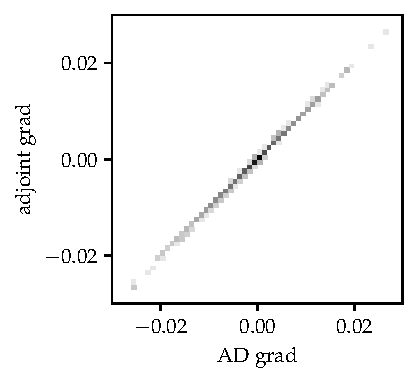
\includegraphics[width=0.5\linewidth]{nn_grads_cmp.pdf}
  \caption{A comparison of adjoint gradients of all parameters in the $f$ and
  $g$ NNs to those by AD.
  This test runs a \pmwd\ simulation of $128^3$ particles, with a $128^3$ mesh
  and 15 time steps.
  The size and time steps of this test case is mainly limited by the memory cost
  of the AD method.
  The two NNs $f$ and $g$ both have two hidden layers of size $[n, n]$, where
  $n$ is the size of the input layer.
  The loss function involves 3 snapshots at $a=(0.6, 0.8, 1)$.
  }
  \label{fig:nn_grads_cmp}
\end{figure*}


%\listofchanges



\end{document}
